%% Direttive TeXworks:
% !TeX root = ./maltoni_niccolo_tesi.tex
% !TEX encoding = UTF-8 Unicode
% !TEX program = arara
% !TEX TS-program = arara
% !TeX spellcheck = it-IT

% arara: pdflatex: { shell: yes, synctex: yes, action: batchmode, options: "-halt-on-error -file-line-error-style" }
% arara: frontespizio
% arara: biber
% arara: pdflatex: { shell: yes, synctex: yes, action: batchmode, options: "-halt-on-error -file-line-error-style" }
% arara: pdflatex: { shell: yes, synctex: yes, action: nonstopmode, options: "-halt-on-error -file-line-error-style" }

% \begin{filecontents*}{\jobname.xmpdata}
% \Title{Progettazione object oriented di un’interfaccia grafica JavaFX per il simulatore Alchemist}
% \Author{Niccolò Maltoni}
% \Keywords{Simulazione\sep JavaFX\sep Interfaccia grafica}
% \Publisher{Università di Bologna}
% \Copyright{Copyright \copyright\ 2017 ``Niccolò Maltoni''}
% \Subject{Lo scopo di questa tesi è la progettazione di un’interfaccia grafica 2D per il simulatore Alchemist. La nuova interfaccia permette di interagire con la simulazione a tempo di esecuzione e di vedere chiaramente rappresentate informazioni su di essa; in particolare, è supportata una struttura modulare di effetti che rende facilmente osservabili determinate entità del sistema ed eventuali loro proprietà. Si è scelto di mantenere un'interfaccia il più possibile user-friendly, mantenendo un design più simile ai simulatori a scopo videoludico per favorire l'utilizzo da parte di utenti inesperti. La libreria grafica utilizzata per l'implementazione è stata JavaFX.}
% \end{filecontents*}

\documentclass[%
    a4paper,            % specifica il formato A4 (default: letter)
    12pt,               % specifica la dimensione del carattere a 12
    % openright,        % serve per aprire i capitoli sulla destra
    openany,            % serve per aprire i capitoli su qualunque pagina
    % oneside,          % serve per impaginare per stampa solo fronte
    twoside,            % serve per impaginare per stampa fronteretro
    % draft,            % evidenzia i punti in cui il testo sborda
    titlepage           % opzione necessaria per il pacchetto frontespizio
]{book}
% \usepackage[a-1b]{pdfx}
\usepackage{a4wide}             % consente di avere più spazio nell'A4

%% ORDINE IMPORTANTE INIZIO %%%%%%%%%%%%
\usepackage[T1]{fontenc}        % serve per impostare la codifica di output del font
\usepackage{textcomp}           % serve per fornire supporto ai Text Companion fonts
\usepackage[utf8]{inputenc}     % serve per impostare la codifica di input del font
\usepackage[
    english,            % utilizza l'inglese come lingua secondaria
    italian             % utlizza l'italiano come lingua primaria
]{%
    babel,                      % serve per scrivere Indice, Capitolo, etc in Italiano
    varioref                    % introduce il comando \vref da usarsi nello stesso modo del comune \ref per i riferimenti
}
\usepackage{lmodern}            % carica una variante Latin Modern prodotto dal GUST
%% ORDINE IMPORTANTE FINE %%%%%%%%%%%%%%

\usepackage{indentfirst}        % serve per avere l'indentazione nel primo paragrafo
\usepackage{setspace}           % serve a fornire comandi di interlinea standard
\usepackage{fancyhdr}           % serve per impaginare bene la tesi
\usepackage{xcolor}             % serve per la gestione dei colori nel testo
\usepackage{graphicx}           % serve per includere immagini e grafici
\usepackage{subfigure}          % serve a creare sottofigure
\usepackage{wrapfig}            % serve per includere figure "wrapped" nel testo
\usepackage[%
    write,              % alternativa a nowrite, crea il file *-frn.tex
    %nowrite,           % alternativa a write, non crea il file *-frn.tex
    standard,           % alternativa a suftesi, crea un frontespizio standard
    %signatures,        % lascia fra i nomi dei relatori lo spazio per le loro firme
    %noadvisor,         % opzione per non mostrare il relatore
    swapnames,          % scambia la posizione dei nomi di relatori e candidato
    normal              % alternativa a sans, utilizza un font "normale"
    %sans,              % alternativa a normal, utilizza un font senza grazie
    %norules,           % eliminano i filetti fra il nome dell’ateneo e quello della facoltà e sopra l’indicazione dell’anno accademico
    %nouppercase,       % disabilita il maiuscoletto nel nome della facoltà
    %noinputenc,        % disabilita la trascrizione dell'inputenc nel preambolo
    %onlyinclude        % disabilita tutte le altre opzioni
]{frontespizio}                 % serve a costruire un buon frontespizio
\usepackage[%
    strict,             % rende tutti gli warning degli errori
    autostyle,          % imposta lo stile in base al linguaggio specificato in babel
    english=american,   % imposta lo stile per l'inglese
    italian=guillemets  % imposta lo stile per l'italiano
]{csquotes}                     % serve a impostare lo stile delle virgolette
\usepackage[%
    maxcitenames=2,     % massimo numero di nomi nelle citazioni
    mincitenames=2,     % minimo numero di nomi nelle citazioni
    maxbibnames=99,     % massimo numero di nomi nella blibliografia
    minbibnames=99,     % minimo numero di nomi nella blibliografia
    style=numeric,      %
    giveninits=true,    %
    backend=biber       % specifica il backend per la bibliografia
]{biblatex}                     % si interfaccia con bibtex e biber per la bibliografia
\addbibresource{biblio.bib}
\usepackage[%
    %notbib,            % rimuove la bibliografia dall'indice
    notindex,           % rimuove l'indice dall'indice
    nottoc,             % rimuove la Table of Contents dall'indice
    notlot,             % rimuove la lista delle tabelle dall'indice
    notlof,             % rimuove la lista delle figure dall'indice
    %chapter,           % "Use chapter-level headings, if possible"
    %section,           % "Use section-level headings, if possible"
    %numbib             % numera il capitolo della bibliografia
    %numindex           % numera il capitolo dell'indice
]{tocbibind}                    % aggiunge cose all'indice
%\usepackage{fncychap}          % serve a personalizzare il formato dei titoli dei capitoli
%\usepackage[]{titlesec}        % una volta definito lo stile nel preambolo con \titleformat formatta i \chapter{}
%\usepackage{enumitem}          % serve a personalizzare liste enumerate, itemize e description
%\usepackage{amssymb}           % abilita i font matematici forniti dall’American Mathematical Society, carica anche {amsfonts}
%\usepackage{mathtools}         % carica {amsmath} e fornisce estensioni per il miglioramento della struttura informativa e della stampa di formule matematiche
%\usepackage{relsize}           % consente di assegnare dimensioni relative con i comandi \smaller e \larger

\onehalfspacing                 % Imposta interlinea a 1,5 ed equivale a \linespread{1,5}

%% TODO capire e poi decidere se inserire o no
%% produce un buon layout con fancyhdr %%%%%%%%%%%%%%%%%%%%%%%%%%%%%%%%%%%%%%
%\pagestyle{fancy}\addtolength{\headwidth}{20pt}
%\renewcommand{\chaptermark}[1]{\markboth{\thechapter.\ #1}{}}
%\renewcommand{\sectionmark}[1]{\markright{\thesection \ #1}{}}
%\cfoot{}
%
%\rhead[\fancyplain{}{\bfseries\leftmark}]{\fancyplain{}{\bfseries\thepage}}
%\lhead[\fancyplain{}{\bfseries\thepage}]{\fancyplain{}{\bfseries\rightmark}}

%% Definisce l'environment abstract per la classe book
\newenvironment{abstract}%
    {\cleardoublepage%
        % \thispagestyle{empty}%
        \null \vfill\begin{center}%
            \bfseries \abstractname \end{center}}%
    {\vfill\null}

% Definisco un nuovo comando per enfatizzare il testo in inglese
\newcommand{\engEmph}[1] {\emph{\foreignlanguage{english}#1}}

\usepackage[htt]{hyphenat}      % Enable hyphenation of TT text
\hyphenation{                   % Permette di sillabare bene le parole
    JavaFX
    Swing
    Micro-systems
    Script
    script
}

\setcounter{secnumdepth}{2}     % Numera fino alla sottosezione nel corpo del testo
\setcounter{tocdepth}{3}        % Numera fino alla sotto-sottosezione nell'indice

\usepackage{hyperref}
\hypersetup{%
    pdfpagemode={UseOutlines},
    hidelinks,          % nasconde i collegamenti (non vengono quadrettati)
    linktoc=all         % inserisce i link nell'indice
    bookmarks=true,
    bookmarksopen,
    pdfstartview={FitH},
    pdfauthor={Niccolò Maltoni},
    pdftitle={Progettazione object oriented di un’interfaccia grafica JavaFX per il simulatore Alchemist}
}
\usepackage[all]{hypcap}        % sistema i problemi di hyperref

% cleveref va anche dopo hyperref
\usepackage[%
    english,italian,    % definizione delle lingue da usare
    nameinlink          % inserisce i link nei riferimenti
]{cleveref}                     % permette di usare riferimenti migliori dei \ref e dei varioref

\begin{document}
    \frontmatter
    \pagenumbering{Roman}
    %% Direttive TeXworks:
% !TeX root = ../../maltoni_niccolo_tesi.tex
% !TEX encoding = UTF-8 Unicode
% !TEX program = arara
% !TEX TS-program = arara
% !TeX spellcheck = it-IT

\begin{frontespizio}
    \Universita{Bologna}
    \Istituzione{%
        Alma Mater Studiorum - Università di Bologna \\%
        Campus di Cesena%
    }
    \Divisione{Scuola di Scienze}
    \Corso[Laurea]{Ingegneria e Scienze Informatiche}
    \Annoaccademico{2016-2017}
    \Titolo{%
        Progettazione object oriented \\%
        di un'interfaccia grafica JavaFX \\%
        per il simulatore Alchemist%
    }
    \Sottotitolo{Tesi in Programmazione ad Oggetti}
    \Candidato{Niccolò~Maltoni}
    \NCandidato{Presentata da}
    \Relatore{Prof.~Mirko~Viroli}
    \Correlatore{Prof.~Danilo~Pianini}
    \Piede{%
        II sessione di laurea \\%
        Anno Accademico 2016 - 2017%
    }
\end{frontespizio}

    %% Direttive TeXworks:
% !TeX root = ../../maltoni_niccolo_tesi.tex
% !TEX encoding = UTF-8 Unicode
% !TEX program = arara
% !TEX TS-program = arara
% !TeX spellcheck = it-IT

%% Direttive Arara:
% arara: pdflatex: { shell: yes, synctex: yes, action: batchmode, options: "-halt-on-error -file-line-error-style" }
% arara: frontespizio
% arara: biber
% arara: pdflatex: { shell: yes, synctex: yes, action: batchmode, options: "-halt-on-error -file-line-error-style" }
% arara: pdflatex: { shell: yes, synctex: yes, action: nonstopmode, options: "-halt-on-error -file-line-error-style" }

\thispagestyle{empty}
\vspace*{20ex}
\begin{flushright}
    \begin{LARGE}
        \textbf{Parole chiave}\\
        \vspace{5ex}
    \end{LARGE}
    \begin{normalsize}
        \textbf{%
            % Alchemist\\%
            % \medskip
            % Simulatore\\%
            % \medskip
            Simulazione\\%
            \medskip
            % Java
            % \medskip
            JavaFX\\%
            \medskip
            Interfaccia grafica\\%
        }
    \end{normalsize}
\end{flushright}
\vfill

    % %% Direttive TeXworks:
% !TeX root = ../../maltoni_niccolo_tesi.tex
% !TEX encoding = UTF-8 Unicode
% !TEX program = arara
% !TEX TS-program = arara
% !TeX spellcheck = it-IT

\clearemptydoublepage
\null\vspace{\stretch{1}}
\begin{flushright}
    \textit{A tutti coloro che mi hanno sostenuto durante questo percorso.}
\end{flushright}
\vspace{\stretch{2}}\null

    \pagestyle{plain}
    %% Direttive TeXworks:
% !TeX root = ../maltoni_niccolo_tesi.tex
% !TEX encoding = UTF-8 Unicode
% !TEX program = arara
% !TEX TS-program = arara
% !TeX spellcheck = it-IT

%% Direttive Arara:
% arara: pdflatex: { shell: yes, synctex: yes, action: batchmode, options: "-halt-on-error -file-line-error-style" }
% arara: frontespizio
% arara: bibtex
% arara: pdflatex: { shell: yes, synctex: yes, action: batchmode, options: "-halt-on-error -file-line-error-style" }
% arara: pdflatex: { shell: yes, synctex: yes, action: nonstopmode, options: "-halt-on-error -file-line-error-style" }

\begin{abstract}
    \addcontentsline{toc}{chapter}{\abstractname}
    Lo scopo di questa tesi verte intorno allo studio del simulatore Alchemist e al fine di progettare un’interfaccia 2D potenziata per l'ambiente grafico relativo alla simulazione. La nuova interfaccia permette di interagire con la simulazione a tempo di esecuzione e di vedere chiaramente rappresentate informazioni su di essa; in particolare, è supportata una struttura modulare di effetti che per rendere ancora più facilmente osservabili determinate entità del sistema ed eventuali loro proprietà. Si è scelto di mantenere un'interfaccia il più possibile \engEmph{user-friendly}, mantenendo un design più simile ai simulatori a scopo videoludico per favorire l'utilizzo da parte di utenti inesperti.

    % TODO analizza risultati

    La seguente trattazione è strutturata su tre capitoli: nel capitolo~\ref{ch:intro} viene introdotto il contesto nel quale il lavoro descritto nella tesi ha preso parte, introducendo il simulatore Alchemist, la sua interfaccia grafica classica e il framework JavaFX; nel capitolo~\ref{ch:contributo} si espone l'intero contributo fornito al progetto, analizzando singolarmente le fasi di analisi dei requisiti, design e progettazione e in ultimo implementazione della nuova interfaccia; infine, il capitolo~\ref{ch:conclusioni} analizza i risultati ottenuti, interpretandoli anche in ottica di miglioramenti futuri.
\end{abstract}

    \tableofcontents

    \mainmatter
    \pagestyle{plain}
    \pagenumbering{arabic}
    \setcounter{page}{1}
    %% Direttive TeXworks:
% !TeX root = ../maltoni_niccolo_tesi.tex
% !TEX encoding = UTF-8 Unicode
% !TEX program = arara
% !TEX TS-program = arara
% !TeX spellcheck = it-IT

%% Direttive Arara:
% arara: pdflatex: { shell: yes, synctex: yes, action: batchmode, options: "-halt-on-error -file-line-error-style" }
% arara: frontespizio
% arara: biber
% arara: pdflatex: { shell: yes, synctex: yes, action: batchmode, options: "-halt-on-error -file-line-error-style" }
% arara: pdflatex: { shell: yes, synctex: yes, action: nonstopmode, options: "-halt-on-error -file-line-error-style" }

\chapter{Introduzione}\label{ch:intro}

    \section{Alchemist}\label{sec:alchemist}
        Alchemist~\cite{alchemistWeb, alchemist2013} è un meta-simulatore estendibile completamente \engEmph{open-source} che esegue su Java Virtual Machine (JVM), nato all'interno del'Università di Bologna e distribuito su licenza GNU GPLv3+ con \engEmph{linking exception}; il codice è reperibile su GitHub\footnote{\url{https://github.com/AlchemistSimulator/Alchemist}}\label{fn:gh}, dove chiunque fosse interessato può collaborare sviluppando nuove estensioni, migliorando funzionalità esistenti e risolvendo possibili bug.

        \subsection{Introduzione ad Alchemist}\label{sub:introAlchemist}
            In generale, una \emph{simulazione}~\cite{des3} è una riproduzione del modo di operare di un sistema o un processo del mondo reale nel tempo.
            L'imitazione del processo del mondo reale è detta \emph{modello}; esso risulta essere una riproduzione più o meno semplificata del mondo reale, che viene aggiornata ad ogni passo di esecuzione della simulazione.

            Alchemist rientra nell'archetipo dei simulatori ad eventi discreti (DES)~\cite{des, des2}: gli eventi sono strettamente ordinati e vengono eseguiti uno alla volta, mentre il tempo viene fatto avanzare parallelamente ad ogni passo (detto \engEmph{tick}).
            L'idea dietro al progetto è quello di riuscire ad avere un framework di simulazione il più possibile generico, in grado di simulare sistemi di tipologia e complessità diverse, mantenendo le prestazioni dei simulatori non generici (come ad esempio quelli impiegati in ambito chimico~\cite{gillespie1976}).

            Per perseguire questo obiettivo, la progettazione dell'algoritmo è partita dal lavoro di Gillespie del 1977~\cite{gillespie1977}, al quale sono state aggiunte diverse modifiche per adattarlo al rinnovato metamodello.

            % TODO aggiungi qualche riferimento al Next Reaction Method (Gibson and Bruck, 2000).

        \subsection{Modello computazionale di Alchemist}\label{sub:modelloComputazionale}
            Il modello (visibile in \figurename~\vref{fig:model}) che costituisce l'architettura base di Alchemist è, come detto, ispirato ad algoritmi tipici della simulazione a scopo di ricerca chimica e, dunque, ne riprende la nomenclatura, seppur con alcune libertà atte ad ottenere una maggiore flessibilità.
            Le entità su cui lavora sono le seguenti:
            \begin{description}

                \item[\engEmph{Molecule}\label{itm:mol}]
                    Una \emph{Molecola} rappresenta il nome dato ad un particolare dato all'interno di un \emph{Nodo}, del quale ne astrae parte dello stato.

                    Un parallelismo con la programmazione imperativa vedrebbe la \emph{Molecola} come un'astrazione del nome di una variabile.

                \item[\engEmph{Concentration}\label{itm:conc}]
                    La \emph{Concentrazione} di una \emph{Molecola} è il valore associato alla proprietà rappresentata dalla \emph{Molecola}.

                    Mantenendo il parallelismo con la programmazione imperativa, la \emph{Concentrazione} rappresenterebbe il valore della variabile.

                \item[\engEmph{Node}\label{itm:node}]
                    Il \emph{Nodo} è un contenitore di \emph{Molecole} e \emph{Reazioni} che risiede all'interno di un \emph{Ambiente} e che astrae una singola entità.

                \item[\engEmph{Environment}\label{itm:env}]
                    L'\emph{Ambiente} è l'astrazione che rappresenta lo spazio nella simulazione ed è l'entità che contiene i nodi.

                    Esso è in grado di fonrire informazioni in merito alla posizione dei \emph{Nodi} nello spazio, alla distanza tra loro e al loro vicinato; opzionalmente, l'\emph{Ambiente} può offrire il supporto allo spostamento dei \emph{Nodi}.

                \item[\engEmph{Linking rule}\label{itm:linkr}]
                    La \emph{Regola di collegamento} è la funzione dello stato corrente dell'\emph{Ambiente} che associa ad ogni \emph{Nodo} un \emph{Vicinato}.

                \item[\engEmph{Vicinato}\label{itm:neigh}]
                    Un \emph{Vicinato} è un'entità costituita da un \emph{Nodo} detto ''centro'' e da un insieme di altri \emph{Nodi} (i ''vicini'').

                    L'astrazione dovrebbe avere un'accezione il più possibile generale e flessibile, in modo da poter modellare qualsiasi tipo di legame di vicinato, non solo spaziale.

                    \begin{figure}[htbp]\label{fig:model}
                        \centering
                        \includegraphics[scale=.4]{img/model}
                        \caption{%
                            La figura, presa dal sito ufficiale~\cite{alchemistWeb}, offre una rappresentazione grafica delle diverse entità. All’interno di un ambiente, che modella il sistema, si trovano i nodi connessi tra loro attraverso dei collegamenti; ogni nodo è composto da reazioni e molecole, ognuna delle quali ha associata una concentrazione.
                        }
                    \end{figure}

                \item[\engEmph{Reaction}\label{itm:react}]
                    Il concetto di \emph{Reazione} è da considerarsi molto più elaborato di quello utilizzato in chimica: in questo caso, si può considerare com un insieme di \emph{Condizioni} sullo stato del sistema, che qualora dovessero risultare vere innescherebbero l'esecuzione di un insieme di \emph{Azioni}.

                    Una \emph{Reazione} è dunque un qualsiasi evento che può cambiare lo stato dell’\emph{Ambiente} e si compone di un insieme di condizioni, una o più azioni e una distribuzione temporale.

                    La frequenza di accadimento può dipendere da:
                    \begin{itemize}
                        \item[--] Un tasso statico;
                        \item[--] Il valore di ciascuna \emph{Condizione};
                        \item[--] Una equazione che combina il tasso statico e il valore delle \emph{Condizioni}, restituendo un ''tasso istantaneo'';
                        \item[--] Una distribuzione temporale.
                    \end{itemize}

                    Ogni \emph{Nodo} è costituito da un insieme (anche vuoto) di \emph{Reazioni}.

                \item[\engEmph{Condition}\label{itm:cond}]
                    Una \emph{Condizione} è una funzione che associa un valore numerico e un valore booleano allo stato corrente di un \emph{Ambiente}.

                \item[\engEmph{Action}\label{itm:act}]
                        Un'\emph{Azione} è una procedura che provoca una modifica allo stato dell'\emph{Ambiente}.
            \end{description}
            
        \subsection{Interfaccia utente classica}\label{sub:prevGui}
            \subsubsection{Esperienza utente}\label{subsub:prevUx}
            \subsubsection{Swing}\label{subsub:swing}
            \subsubsection{Gli effetti e l'interfaccia \texttt{Effect}}\label{subsub:effect}
    \section{JavaFX}\label{sec:jfx}
        \subsection{Introduzione a JavaFX}\label{sub:jfxIntro}
        \subsection{Il framework JavaFX}\label{sub:jfxFramework}
        \subsection{Struttura di una Applicazione JavaFX}\label{sub:jfxStruttura}
        \subsection{Vantaggi di JavaFX su Swing}\label{sub:jfxVantaggi}
    \section{Interfaccia JavaFX per Alchemist: motivazioni}\label{sec:motivi}

    %% Direttive TeXworks:
% !TeX root = ../maltoni_niccolo_tesi.tex
% !TEX encoding = UTF-8 Unicode
% !TEX program = arara
% !TEX TS-program = arara
% !TeX spellcheck = it-IT

%% Direttive Arara:
% arara: pdflatex: { shell: yes, synctex: yes, action: batchmode, options: "-halt-on-error -file-line-error-style" }
% arara: frontespizio
% arara: biber
% arara: pdflatex: { shell: yes, synctex: yes, action: batchmode, options: "-halt-on-error -file-line-error-style" }
% arara: pdflatex: { shell: yes, synctex: yes, action: nonstopmode, options: "-halt-on-error -file-line-error-style" }

\chapter{Contributo}\label{ch:contributo}
  \section{Analisi dei requisiti}\label{sec:analisi}
    \subsection{Requisiti funzionali}\label{sub:funzionali}
    \subsection{Requisiti non funzionali}\label{sub:nonFunzionali}
  \section{Fonti d'ispirazione}\label{sec:ispirazione}
    \subsection{Simulatori a scopo videoludico}\label{sub:videogame}
      \subsubsection{Universe Sandbox}\label{subsub:us1}
      \subsubsection{Universe Sandbox 2}\label{subsub:us2}
      \subsubsection{SimCity}\label{subsub:simcity}
    \subsection{Material Design}\label{sub:material}
  \section{Design dell'interfaccia}\label{sec:design}
  \section{Progettazione}\label{sec:progettazione}
      \subsection{La barra inferiore}\label{sub:barra}
      \subsection{La struttura a drawer}\label{sub:drawer}
      \subsection{L'architettura degli effetti}\label{sub:effetti}
      % \subsubsection{I gruppi di effetti e l'interfaccia \texttt{EffectGroup}}\label{subsub:effectGroup}
      % \subsubsection{I singoli effetti e l'interfaccia \texttt{EffectFX}}\label{subsub:effectFX}
      % \subsubsection{Caricamento, salvataggio e modifica di gruppi di effetti}\label{subsub:serializzazione}
  \section{Dettagli implementativi}\label{sec:dettagli}
    % \subsection{Librerie utilizzate}\label{sub:lib}
    % \subsection{Gestione della concorrenza}\label{sub:concorrenza}

    %% Direttive TeXworks:
% !TeX root = ../maltoni_niccolo_tesi.tex
% !TEX encoding = UTF-8 Unicode
% !TEX program = arara
% !TEX TS-program = arara
% !TeX spellcheck = it-IT

%% Direttive Arara:
% arara: pdflatex: { shell: yes, synctex: yes, action: batchmode, options: "-halt-on-error -file-line-error-style" }
% arara: frontespizio
% arara: biber
% arara: pdflatex: { shell: yes, synctex: yes, action: batchmode, options: "-halt-on-error -file-line-error-style" }
% arara: pdflatex: { shell: yes, synctex: yes, action: nonstopmode, options: "-halt-on-error -file-line-error-style" }

\chapter{Conclusioni}\label{ch:conclusioni}
    \section{Risultati}\label{sec:risultati}
        L'obiettivo di questa tesi era quello di realizzare un'interfaccia grafica per l'ambiente di simulazione di Alchemist che sostituisse la precedente e si andasse ad integrare con i recenti contributi dati ad altre sezioni della GUI del software, andando a fornire una esperienza utente più semplice e gradevole anche per i meno esperti.

        L'interfaccia, realizzata con la libreria JavaFX, ha comportato un restyling completo a livello estetico e una reimplementazione di numerose parti del codice; i requisiti sono quasi completamente soddisfatti, fatta eccezione per l'ambiente di simulazione (\textbf{\texttt{e tutto il resto che al momento manca [ndr.]}}).
        Nonostante quest'ultima mancanza non permetta il completo abbandono dell'interfaccia precedente, il codice realizzato adempie con correttezza ai compiti per cui è stato scritto, dunque l'implementazione può considerarsi riuscita.

        \textbf{\texttt{[Continua...]}}

    \section{Lavori futuri}\label{sec:futuro}
        \textbf{\texttt{[...]}}


    % %% Direttive TeXworks:
% !TeX root = ../maltoni_niccolo_tesi.tex
% !TEX encoding = UTF-8 Unicode
% !TEX program = arara
% !TEX TS-program = arara
% !TeX spellcheck = it-IT

\appendix
    % \chapter{Codice relativo all'interfaccia classica}\label{appendix:old}
        % \section{L'interfaccia \texttt{Effect}}\label{appendix:effect}
            % TODO codice

    % \chapter{Codice relativo al contributo}\label{appendix:new}
        % \section{L'interfaccia \texttt{EffectFX}}\label{appendix:effectfx}
            % TODO codice
        \chapter{L'interfaccia \texttt{EffectFX}}\label{appendix:effectfx}
            % TODO UML

        % \section{L'interfaccia \texttt{EffectGroup}}\label{appendix:effectgroup}
            % TODO codice

        %\section{Implementazioni di \texttt{EffectFX} e Proprietà serializzabili}\label{appendix:effectsAndProps}
            % TODO codice
        \chapter{Implementazioni di \texttt{EffectFX} e Proprietà serializzabili}\label{appendix:effectsAndProps}
            % TODO UML
            % \begin{figure}[htbp]
                % \centering
                % \includegraphics[scale=0.7]{img/EffectAndPropertiesUML}
                % \caption{Il diagramma UML delle classi mostra le relazioni tra gli effetti implementati e le proprietà custom utilizzate}
            % \end{figure}


    \backmatter
    %% Direttive TeXworks:
% !TeX root = ../../maltoni_niccolo_tesi.tex
% !TEX encoding = UTF-8 Unicode
% !TEX program = arara
% !TEX TS-program = arara
% !TeX spellcheck = it-IT

%% Direttive Arara:
% arara: pdflatex: { shell: yes, synctex: yes, action: batchmode, options: "-halt-on-error -file-line-error-style" }
% arara: frontespizio
% arara: biber
% arara: pdflatex: { shell: yes, synctex: yes, action: batchmode, options: "-halt-on-error -file-line-error-style" }
% arara: pdflatex: { shell: yes, synctex: yes, action: nonstopmode, options: "-halt-on-error -file-line-error-style" }

% per quanto non citato esplicitamente, Effective Java (2nd Edition) di Joshua Bloch ha dato il suo contributo alla scrittura del codice
\nocite{Bloch:2008:EJ:1377533}
\printbibliography[heading=bibintoc]

    % \listoffigures
    % \listoftables
    % %% Direttive TeXworks:
% !TeX root = ../../maltoni_niccolo_tesi.tex
% !TEX encoding = UTF-8 Unicode
% !TEX program = arara
% !TEX TS-program = arara
% !TeX spellcheck = it-IT

\chapter*{Ringraziamenti}
% \addcontentsline{toc}{chapter}{Ringraziamenti}
Un sincero ringraziamento va a tutti coloro che mi hanno aiutato in vario modo a raggiungere questo importante traguardo.
Ringrazio il professor Mirko Viroli e il professor Danilo Pianini per tutto l’aiuto datomi per realizzare questo progetto, sia durante l'attività sperimentale che per la realizzazione dell'elaborato finale.
Ringrazio anche gli amici che mi sono stati accanto durante questi mesi, ma soprattutto un particolare grazie ai miei genitori che mi sostengono da sempre.

\end{document}
